%%%%%%%%%%%%%%%%%%%%%%%%%%%%%%%%%%%%%%%%%%%%%%%%%%%%%%%%%%%%%%%%%%%%%%%%%%%%%%%%%%%%%%%%%%%%%%%%%%%%%%%
%%%%%%%%%%%%%% Template de Artigo Adaptado para Trabalho de Diplomação do ICEI %%%%%%%%%%%%%%%%%%%%%%%%
%% codificação UTF-8 - Abntex - Latex -  							     %%
%% Autor:    Fábio Leandro Rodrigues Cordeiro  (fabioleandro@pucminas.br)                            %% 
%% Co-autores: Prof. João Paulo Domingos Silva, Harison da Silva e Anderson Carvalho		     %%
%% Revisores normas NBR (Padrão PUC Minas): Helenice Rego Cunha e Prof. Theldo Cruz                  %%
%% Versão: 1.1     18 de dezembro 2015                                                               %%
%%%%%%%%%%%%%%%%%%%%%%%%%%%%%%%%%%%%%%%%%%%%%%%%%%%%%%%%%%%%%%%%%%%%%%%%%%%%%%%%%%%%%%%%%%%%%%%%%%%%%%%
\section{\esp Introdução}

No início do século XVIII, especula-se que, na cidade russa de Königsberg, eram constituídas quatro áreas, as quais eram separadas pelo Rio Pregel. No entanto, o deslocamento dos cidadãos era complexo devido a utilização de barcos para tal. Assim sendo, foram construídas sete pontes conforme ilustrado na figura 1, para auxiliar na locomoção destes entre as ilhas e suas margens. Contudo, o trajeto ainda se tornava árduo e tais pessoas da época começaram a se questionar se era possível cruzar as pontes apenas uma vez e, se possível, retornar ao ponto inicial.

\begin{figure}[ht]
	\centering	
	\caption[\hspace{0.1cm}Esboço da cidade de Königsberg.]{Esboço da cidade de Königsberg}
	\vspace{-0.4cm}
	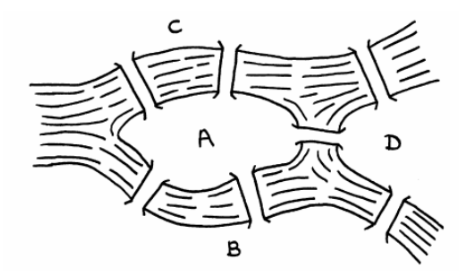
\includegraphics[width=0.6\textwidth]{figuras/cidade.png}
	 \vspace{-0.2cm}
	\\\textbf{\footnotesize Fonte: Hopkins; Wilson, 2004, p. 198}
	\label{fig:figura1}
\end{figure}

O grande matemático suiço Leonhard Euler, chega à Rússia no ano de 1730 para exercer o cargo de Filosofia Natural na Academia de Ciências de São Petersburgo. No entanto, após três anos tornou-se o principal matemático da academia com a saída de Daniel Bernoulli.

Com sua ascensão, o prefeito próximo a cidade de Königsberg enviou-lhe uma carta datada de 09 de março de 1736 em nome de Heinrich Kiihn, um matemático local que explica a questão das pontes. Intrigado com a questão Euler envia uma carta a Giovanni Jacopo Marinoni, um matemático e engenheiro italiano repassando a questão e dizendo em sua carta:

\begin{citacaodireta}
Um problema me foi apresentado sobre uma ilha na cidade de Konigsberg, cercada por um rio, atravessado por sete pontes, e foi me perguntado se alguém poderia atravessar as pontes separadas em uma caminhada contínua de tal forma que cada ponte fosse atravessada apenas uma vez. Fui informado que até então ninguém havia demonstrado a possibilidade de fazer isso, ou mostrado que é impossível. Esta questão é tão banal, mas pareceu-me digno de atenção em que nem a geometria, álgebra, ou mesmo a arte de contar foram suficientes para resolvê-lo (HOPKINS; WILSON, 2004, p. 201).
\end{citacaodireta}

Euler então monta um modelo matemático representando o mapa da cidade, associando cada ilha a um ponto e cada ponte como uma linha que interliga esses pontos.  Desta forma originalizando a Teoria dos Grafos com base na figura 2 ilustrada abaixo:

\begin{figure}[ht]
	\centering	
	\caption[\hspace{0.1cm}Grafo que representa a cidade de Königsberg.]{Grafo que representa a cidade de Königsberg}
	\vspace{-0.4cm}
	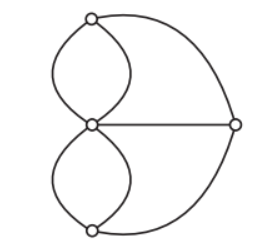
\includegraphics[width=0.3\textwidth]{figuras/grafo-cidade.png}
	 \vspace{-0.2cm}
	\\\textbf{\footnotesize Fonte: Desenvolvido pelo autor}
	\label{fig:figura1}
\end{figure}

Esta figura representa seus pontos como vértices e suas ligações como arestas, denominando um grafo. Euler percebe durante seu raciocínio que existem vértices com exatamente três arestas incidentes. Entretanto, os cidadãos gostariam de atravessar cada ponte apenas uma única vez, mas cada vértice deveria conter um número par de arestas, tornando impossível o percurso seguindo as restrições da população.

Com a resolução desta questão que indica que se e somente, se o grafo possuir números pares de arestas é possível passar uma única vez pelo caminho. Euler, então envia sua resposta ao prefeito em 03 de abril de 1736 da seguinte forma:

\begin{citacaodireta}
Assim você vê, mais nobre senhor, como este tipo de solução tem pouca relação com a matemática, e eu não entendo por que você espera que um matemático possa produzi-la, ao invés de qualquer outra pessoa, já que a solução baseia-se na razão e sua descoberta não depende de qualquer princípio matemático. Devido a isso, eu não sei por que questões comuns que têm tão pouca relação com a matemática são resolvidas mais rapidamente pelos matemáticos do que por outros (HOPKINS; WILSON, 2004, p. 201).
\end{citacaodireta}

Apesar de não vincular sua resolução do problema à matemática, Euler se interessou em divulgar sua análise para a comunidade científica da época. Na qual foi homenageado com parte de seu nome no Teorema dos Caminhos Eulerianos. Passado algum tempo começaram a surgir novos problemas, como o do Caixeiro Viajante, o das Quatro Cores e o do Carteiro Chinês, que permitiram o desenvolvimento da Teoria dos Grafos.

\section{\esp CONCEITOS SOBRE GRAFOS}

Como toda teoria matemática, a Teoria dos Grafos contém diversas nomenclaturas e termos técnicos. Nesta seção são apresentadas algumas de suas definições principais para o entendimento completo deste estudo.

\subsection{\esp Estruturas de um Grafo}

Grafo é uma representação abstrata de um conjunto de objetos e das relações existentes entre eles. Podendo ser descrito como um par de G(V, A) onde V é um conjunto não vazio de objetos denominados vértices e A é um conjunto de pares não ordenados de V, chamado arestas. Por exemplo, no grafo apresentado na figura 3 é apresentado um mapa de estradas e cidades.

\begin{figure}[ht]
	\centering	
	\caption[\hspace{0.1cm}Exemplo de um grafo.]{Exemplo de um grafo}
	\vspace{-0.4cm}
	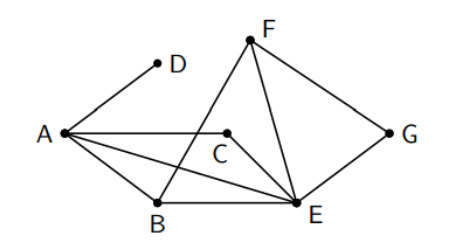
\includegraphics[width=0.3\textwidth]{figuras/exemplo-grafo.png}
	 \vspace{-0.2cm}
	\\\textbf{\footnotesize Fonte: Desenvolvido pelo autor}
	\label{fig:figura1}
\end{figure}

Pode-se destacar que dependendo da aplicação, as arestas do grafo podem ou não ser orientadas, ligar um vértice a ele próprio e ainda ter um peso (numérico) associado.

Grafos não orientados, ou simplesmente grafos, são compostos por dois vértices que são adjacentes se existir uma aresta conectando-os, ao passo que uma aresta é incidente aos vértices que ela conecta. 

\begin{figure}[ht]
	\centering	
	\caption[\hspace{0.1cm}Grafo não direcionado.]{Grafo não direcionado}
	\vspace{-0.4cm}
	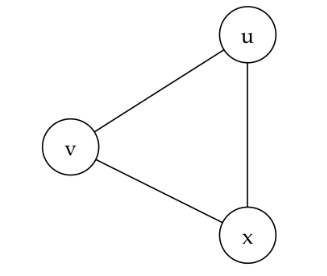
\includegraphics[width=0.3\textwidth]{figuras/grafo-nao-direcionado.png}
	 \vspace{-0.2cm}
	\\\textbf{\footnotesize Fonte: Desenvolvido pelo autor}
	\label{fig:figura1}
\end{figure}

Grafos orientados ou também conhecidos como dígrafos, dizemos que um vértice X é adjacente a um Y se, e somente se, (X,Y) pertence ao conjunto de arestas do grafo. No caso de incidência em grafos orientados, há de se considerar que a aresta (X,Y) é incidente somente em Y, enquanto a aresta (Y,X) incide em X.

\begin{figure}[ht]
	\centering	
	\caption[\hspace{0.1cm}Grafo direcionado ou dígrafo.]{Grafo direcionado ou dígrafo}
	\vspace{-0.4cm}
	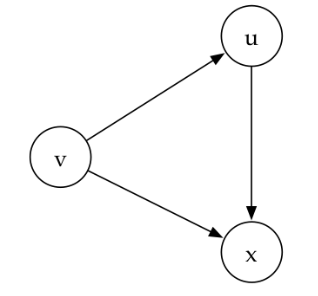
\includegraphics[width=0.3\textwidth]{figuras/grafo-direcionado.png}
	 \vspace{-0.2cm}
	\\\textbf{\footnotesize Fonte: Desenvolvido pelo autor}
	\label{fig:figura1}
\end{figure}

Grafos ponderados, possuem atribuição de pesos em suas arestas. São utilizados para determinar qual o melhor trajeto a adotar dado o problema. Supondo que para ir de um lugar para outro existem diversas estradas em que cada uma possui um pedágio e deseja-se escolher a estrada com menor valor de pedágio para chegar até o destino. O grafo da figura 6 exemplifica essa suposição.

\begin{figure}[ht]
	\centering	
	\caption[\hspace{0.1cm}Grafo ponderado.]{Grafo ponderado}
	\vspace{-0.4cm}
	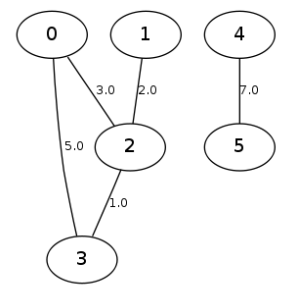
\includegraphics[width=0.3\textwidth]{figuras/grafo-ponderado.png}
	 \vspace{-0.2cm}
	\\\textbf{\footnotesize Fonte: Desenvolvido pelo autor}
	\label{fig:figura1}
\end{figure}


\section{\esp Desenvolvimento}

Todo título de seção ou subseção deverá ser seguido de texto.
Para as seções textuais utilizar numeração progressiva em algarismos arábicos, limitada até a seção quinária 
(NBR 6024/2003) da ABNT. Devem ser diferenciadas utilizando os recursos gráficos abaixo \cite{manualpuc}.
Os títulos das seções primárias devem ser em caixa alta, negrito, tamanho 12.

\subsection{\esp Seção secundária}

Os títulos das seções secundárias terão caixa baixa, negrito, tamanho 12.

\subsubsection{\esp Seção terciária}

Caixa baixa, itálico, negrito, tamanho 12.

\subsubsubsection{\esp Seção quartenária}
 
 Caixa baixa, sublinhado, negrito, tamanho 12.
 
 \subsubsubsubsection{\esp Seção quinária}
 
 Nas seções quinárias, deve ser usado caixa baixa, sem negrito, tamanho 12.

\section{\esp Elementos flutuantes}

Elementos inseridos no texto como imagens, tabelas, algoritmos etc.
Recomenda-se a colocação das ilustrações de forma centralizada, dentro das margens. 
Caso não seja possível, em \citeonline{manualpuc} recomenda-se utilizar recursos como: 
 a) utilizar letras com tamanho menor ao padrão do texto; a) imprimir a ilustração no sentido vertical; 
 c) imprimir em folha A3 ou superior e dobrá-la até atingir o tamanho da folha A4. 

Nas normas da PUC é afirmado a necessidade de se observar que todos os elementos flutuantes inseridos devem ter a formatação básica:

\begin{enumerate} 
 \item [a)] Título centralizado localizado na parte superior; 
 \item [a)] Fonte em tamanho 10 na parte inferior;
 \item [c)] Devem ser inseridas o mais próximos do texto que as referenciam.
\end{enumerate}


\subsection{\esp Inserções de ilustrações}

As ilustrações devem ser inseridas seguindo o exemplo da Figura \ref{fig:figura1}. 
% Figura
\begin{figure}[ht]
	\centering	
	\caption[\hspace{0.1cm}Grade Computacional.]{Uma Grade Computacional como fonte transparente}
	\vspace{-0.4cm}
	\includegraphics[width=0.6\textwidth]{figuras/grade-comp.png}
	% Caption centralizada
% 	\captionsetup{justification=centering}
	% Caption e fonte 
	 \vspace{-0.2cm}
	\\\textbf{\footnotesize Fonte: \citeonline{cap-livro} }
	\label{fig:figura1}
\end{figure}
\vspace{-0.5cm}

\subsection{\esp Inserção de tela de software}

Nos casos de telas de \textit{software}, devem ser inseridas como figuras, e referenciadas no texto
como na Figura \ref{fig:tela1}. Além disso, é necessário que seja citada no texto a empresa desenvolvedora. 

% Figura
\begin{figure}[!ht]
	\centering	
	\caption[\hspace{0.1cm}Exemplo de tela de software.]{Exemplo de tela de software}
	  \vspace{-0.4cm}
	\includegraphics[width=.8\textwidth]{figuras/tela1.png}
	% Caption centralizada
% 	\captionsetup{justification=centering}
	% Caption e fonte
	 \vspace{-0.3cm}
	\\\textbf{\footnotesize Fonte: \citeonline{tela1}}
	\label{fig:tela1}
\end{figure}

%Utilize o \newpage no caso de quando a figura ficar sobreposta por um texto, como é o caso que acontece na figura anterior
%Retire o \newpage para verificar esse exemplo
\newpage
%-------------------------------------------------------------------------------------------------------------------------

\subsection{\esp Inserção de gráficos e mapas}

O gráfico é um tipo de ilustração que deve conter todos os elementos citados e também a descrição de seu título
diferenciando-o das figuras da mesma forma que no Gráfico 1. 

\begin{center}
	\centering	
 	\textbf{Gráfico 1 - Exemplo de um gráfico} \\
%  	  \vspace{0.cm}
	\includegraphics[width=0.7\textwidth]{figuras/access.png}
	% Caption centralizada
% 	\captionsetup{justification=centering}
	% Caption e fonte
	 \vspace{-0.3cm}
	\\\textbf{\footnotesize Fonte: \citeonline{tese}}
	\label{grafico1}
\end{center}

A mesma regra se aplica para mapas, que devem ser adicionados seguindo as regras de apresentação já mostradas. No caso específico,
o título e a numeração, também como os gráficos, devem começar do numeral ``1'' depois da marcação ``Mapa'' seguido do nome do elemento.
Exemplo: \textbf{Mapa 1 - Exemplo de um Mapa}.

 \subsection{\esp Tabelas}

As tabelas devem ser abertas nas laterais, com espaços verticais separando
as colunas e sem espaços horizontais, exceto na
separação do cabeçalho. Um exemplo é a Tabela \ref{tab:tabela1}. 

% Tabela
\begin{table}[htb]
	\centering
	\caption{\hspace{0.1cm} Exemplo de uma tabela}
	\vspace{-0.3cm} % espaço entre titulo e tabela
	\label{tab:tabela1}
	% Conteúdo da tabela
	\begin{tabular}{l|c|c}
  \hline
    \textbf{Imagem}	& \textbf{transferência} & \textbf{tempo} \\
    \hline
     estação 1	& 7,72 MB/s &  1:22:18 \\
     estação 2	& 7,72 MB/s &  1:22:17 \\
     estação 3	& 7,59 MB/s & 1:24:25 \\
     estação 4  & 7,53 MB/s & 1:43:27 \\
     estação 5	& 6,14 MB/s  &  1:24:41 \\
     estação 6  &  7,50 MB/s & 1:23:53 \\
     estação 7  & 7,58 MB/s  &  1:24:02 \\
     estação 8  & 7,8 MB/s  &  1:29:06 \\
     estação 9  & 7,9 MB/s  &  1:30:05 \\
     estação 10 & 8,0 MB/s  &  1:32:03 \\
     \hline
 \end{tabular}
 	\vspace{.1cm}  %espaço entre tabela e fonte
	\small
	% Fonte
	{\footnotesize\\ \textbf{Fonte: \citeonline{monog-fabio}}}
\end{table}
   

\subsection{\esp Inserção de algoritmos}

Para inserir um algoritmo, utilizar o exemplo do Algoritmo  \ref{alg:rnagenerica}.
Todos os algoritmos devem ser inseridos como figura, indicada por nome e  fonte. Caso 
forem de própria autoria, isso deverá ser mencionado na fonte, como elaboração feita pelos autores.

% algoritmo
% \begin{figure}[ht]
\begin{center}	
	% Arquivo da figura
% 	\caption[\hspace{0.1cm} Texto da figuras.]{Algorítmo CAC RD Neural}
         \textbf{Algoritmo 1 -  CAC RD Neural}
	\vspace{-0.3cm}
\begin{minipage}[ht]{13cm}
\begin{algorithm}[H]
  \footnotesize
  \caption{CAC-RD Neural}
  \label{alg:rnagenerica}
  \begin{algorithmic}[1]
      \STATE \textbf{Entrada:} Requisição da chamada
    \STATE \textbf{Saída:} Aceitação ou bloqueio da solicitação
    
    \STATE Preenche o vetor de $attributes.size+1$ atributos com os valores dos atributos, sendo a primeira posição do vetor preenchida com o valor 1
		\STATE $hidden\_layer\_size =  attributes.size*2+1;$

    \FOR{$i$ = 1 to $attributes.size+1$}
    	\STATE \textbf{normalizar}($Entrada_i$)
    \ENDFOR

		\STATE $double [] net = new double [hidden\_layer\_size];$
    \STATE $net = hidden\_layer\_weights * attributes;$
   	\FOR{$i$ = 0 to hidden\_layer\_size}
			\STATE $net [i] = 1.0 / (1.0 + exp((-1.0)*net[i]));$
		\ENDFOR

		\STATE $double [] ipVector = new double [hidden\_layer\_size+1];$
    \STATE $ipVector [0] = 1.0;$
   	\FOR{$i$ = 1 to $hidden\_layer\_size+1$}
			\STATE $ipVector [i] = net [i-1];$
		\ENDFOR
		
		\STATE $output = output\_layer\_weights *  ipVector;$
    \STATE output = \textbf{desnormalizar}(Saída)
    \STATE \textbf{net\_update} (requisition);
    
    \STATE \textbf{Retorna} output; FIM
  \end{algorithmic}
\end{algorithm}
% \vspace{-0.3cm} % espaço entre algoritmo e fonte

\small \centering \textbf{\footnotesize Fonte: \citeonline{mestrado}.}
\end{minipage}
\end{center}
% \end{figure}


\subsection{\esp Conclusão}

Discussão dos resultados obtidos na pesquisa. É onde se colocam as observações do autor. 
Poderá também apresentar sugestões de novas linhas de estudo.

A conclusão deve estar de acordo com os objetivos do trabalho.

A conclusão não deve apresentar citações ou interpretações de outros autores.
